\begin{pa} \label{PA:9.8} In earlier investigations, we have used
  integration to calculate quantities such as area, volume, mass, and
  work.  We are now interested in determining the 
  length of a space curve.

  Consider the smooth curve in 3-space defined by the vector-valued
  function
    \[\vr(t) = \langle x(t), y(t), z(t) \rangle = \langle \cos(t), \sin(t), t \rangle\]
    for $t$ in the interval $[0,2\pi]$. Pictures of the graph of $\vr$ are shown in Figure \ref{F:9.8.Arc_length}.
  We will use the integration process to calculate the length of this curve. In this situation we partition the interval $[0,2\pi]$ into $n$ subintervals of equal length and let $0 = t_0 < t_1 < t_2 < \cdots < t_n = b$ be the endpoints of the subintervals. We then approximate the length of the curve on each subinterval with some related quantity that we can compute. In this case, we approximate the length of the curve on each subinterval with the length of the segment connecting the endpoints. Figure \ref{F:9.8.Arc_length} illustrates the process in three different instances using increasing values of $n$. 
\begin{figure}[ht]
\begin{center}
%\begin{minipage}{2.5in}
%\begin{center}
\resizebox{!}{1.5in}{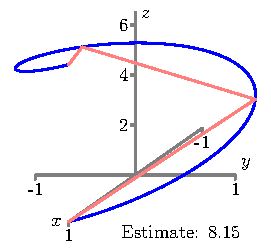
\includegraphics{figures/fig_9_8_length_animate_02.pdf}} \hspace{0.25in} \resizebox{!}{1.5in}{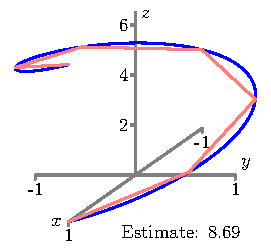
\includegraphics{figures/fig_9_8_length_animate_05.pdf}} \hspace{0.25in} \resizebox{!}{1.5in}{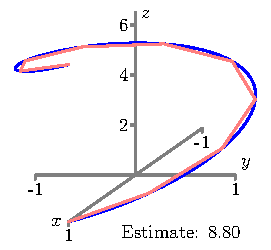
\includegraphics{figures/fig_9_8_length_animate_08.pdf}}
%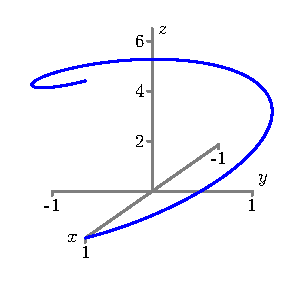
\includegraphics{figures/fig_9_8_length_1.eps}
%\end{center}
%\caption{The graph of $\vr$.}
%\label{F:9.8.Arc_length_3d}
%\end{minipage} \hspace{0.5in}
%\begin{minipage}{2.5in}
%\begin{center}
%\resizebox{!}{2.25in}{\animategraphics[controls,trim=0cm 0.0cm 0.25cm 1.5cm]{4}{9_8_AL3D_}{01}{20}}
%\animategraphics[controls]{2}{figures/fig_9_8_length_animate_}{00}{24}
\end{center}
\caption{Approximating the length of the curve with $n=3$, $n=6$, and $n=9$.}
\label{F:9.8.Arc_length}
%\label{F:9.8.Arc_length_3d_animation}
%\end{minipage}
%\end{center}
\end{figure}
%crop graphics in animate trim=<left> <bottom> <right> <top>, add, clip with \includegraphics
%Write the coordinates of the points on the curve determined by the endpoints of the interval $[x_{i-1},x_i]$.
    \ba
	\item Write a formula for the length of the line segment that connects the endpoints of the curve on the $i$th subinterval $[t_{i-1},t_i]$. (This length is our approximation of the length of the curve on this interval.) 
	
    \item Use your formula in part (a) to write a sum that adds all of the approximations to the lengths on each subinterval.

    \item What do we need to do with the sum in part (b) in order to obtain the exact value of the length of the graph of $\vr(t)$ on the interval $[0,2\pi]$?

    \ea


\end{pa} 


\begin{activitySolution}
   \ba
	\item The length of the line segment connecting the points $\vr(t_{i-1})$ and $\vr(t_i)$ is given by the distance formula
\[\sqrt{(x_i-x_{i-1})^2+(y_{i}-y_{i-1})^2 + (z_{i}-z_{i-1})^2}.\]

    \item We add the lengths given in part (b) to obtain the sum
\[\sum_{i=1}^n \sqrt{(x_i-x_{i-1})^2+(y_{i}-y_{i-1})^2 + (z_{i}-z_{i-1})^2}\]
that approximates the total length of the graph of $\vr(t)$ on the interval $[0,2 \pi]$.

    \item We must take the limit of the sum as $n$ goes to infinity.


    \ea
\end{activitySolution}


\afterpa 